\documentclass[paper=a4, fontsize=11pt]{report} % A4 paper and 11pt font size
\usepackage[utf8]{inputenc}
\usepackage[T1]{fontenc} % Use 8-bit encoding that has 256 glyphs
\usepackage[english]{babel} % English language/hyphenation
\usepackage{amsmath,amsfonts,amsthm} % Math packages


\usepackage{graphicx}
\usepackage{caption}
\usepackage{subcaption}

\usepackage{siunitx}
\usepackage{float}
\usepackage{subfiles} %Enables inclusions of files that can compile standalone

\usepackage{todonotes}
\usepackage{wrapfig}

\usepackage[nottoc]{tocbibind}

\usepackage[backend=bibtex]{biblatex}
\bibliography{bibtexlibs}

\usepackage{sectsty} % Allows customizing section commands
\allsectionsfont{\centering \normalfont\scshape} % Make all sections centered, the default font and small caps

\usepackage{array}
\newcolumntype{L}[1]{>{\raggedright\let\newline\\\arraybackslash\hspace{0pt}}m{#1}}
\renewcommand{\arraystretch}{1.5} % increase vertical spacing in table cells

\usepackage{parskip}
\setlength{\parindent}{0pt}

\usepackage{tabularx}

\usepackage{fancyhdr} % Custom headers and footers
\pagestyle{fancyplain} % Makes all pages in the document conform to the custom headers and footers
\fancyhead[L]{} % No page header - if you want one, create it in the same way as the footers below
\fancyfoot[L]{} % Empty left footer
\fancyfoot[C]{} % Empty center footer
\fancyfoot[R]{\thepage} % Page numbering for right footer
\renewcommand{\headrulewidth}{0pt} % Remove header underlines
\renewcommand{\footrulewidth}{0pt} % Remove footer underlines
\setlength{\headheight}{13.6pt} % Customize the height of the header

\usepackage{hyperref}
\hypersetup{
    colorlinks,
    citecolor=black,
    filecolor=black,
    linkcolor=black,
    urlcolor=black
}

%\usepackage{refcheck}

\fancypagestyle{firststyle}
{
  \fancyhf{}
  \fancyfoot[R]{\thepage}
}

\numberwithin{equation}{section} % Number equations within sections (i.e. 1.1, 1.2, 2.1, 2.2 instead of 1, 2, 3, 4)
\numberwithin{figure}{section} % Number figures within sections (i.e. 1.1, 1.2, 2.1, 2.2 instead of 1, 2, 3, 4)
\numberwithin{table}{section} % Number tables within sections (i.e. 1.1, 1.2, 2.1, 2.2 instead of 1, 2, 3, 4)

%------ Listings --------------
\usepackage{color}
\definecolor{light-gray}{gray}{0.95}
\definecolor{orange}{rgb}{1, 0.5, 0}
\definecolor{backcolor}{rgb}{0.95,0.95,0.92}
\usepackage{listings}
\usepackage{../main/assembly}

\lstnewenvironment{assembly}[1][]%
{\minipage{\linewidth}
\lstset{ %
language=assembly,  % choose the language of the code
basicstyle=\footnotesize,       % the size of the fonts that are used for the code
numbers=left,                   % where to put the line-numbers
numberstyle=\footnotesize,      % the size of the fonts that are used for the line-numbers
stepnumber=1,                   % the step between two line-numbers. If it is 1 each line will be numbered
resetmargins=true,              % reset line numbers
numbersep=5pt,                  % how far the line-numbers are from the code
backgroundcolor=\color{backcolor},  % choose the background color. You must add \usepackage{color}
showspaces=false,               % show spaces adding particular underscores
showstringspaces=false,         % underline spaces within strings
showtabs=false,                 % show tabs within strings adding particular underscores
tabsize=2,                      % sets default tabsize to 2 spaces
captionpos=b,                   % sets the caption-position to bottom
breaklines=true,                % sets automatic line breaking
breakatwhitespace=false,        % sets if automatic breaks should only happen at whitespace
escapeinside={\%*}{*)},         % if you want to add a comment within your code
identifierstyle=\color{blue},
stringstyle=\color{orange},
#1
}}%
{\endminipage}

\lstnewenvironment{c-code}[1][]%
{\minipage{\linewidth}
\lstset{ %
language=C,  % choose the language of the code
basicstyle=\footnotesize,       % the size of the fonts that are used for the code
numbers=left,                   % where to put the line-numbers
numberstyle=\footnotesize,      % the size of the fonts that are used for the line-numbers
stepnumber=1,                   % the step between two line-numbers. If it is 1 each line will be numbered
resetmargins=true,              % reset line numbers
numbersep=5pt,                  % how far the line-numbers are from the code
backgroundcolor=\color{backcolor},  % choose the background color. You must add \usepackage{color}
showspaces=false,               % show spaces adding particular underscores
showstringspaces=false,         % underline spaces within strings
showtabs=false,                 % show tabs within strings adding particular underscores
tabsize=2,                      % sets default tabsize to 2 spaces
captionpos=b,                   % sets the caption-position to bottom
breaklines=true,                % sets automatic line breaking
breakatwhitespace=false,        % sets if automatic breaks should only happen at whitespace
escapeinside={\%*}{*)},         % if you want to add a comment within your code
identifierstyle=\color{blue},
stringstyle=\color{orange},
#1
}}%
{\endminipage}


%----------------------------------------------------------------------------------------
%   TITLE SECTION
%----------------------------------------------------------------------------------------

\newcommand{\horrule}[1]{\rule{\linewidth}{#1}} % Create horizontal rule command with 1 argument of height

\title{ 
\normalfont \normalsize 
\textsc{Norwegian University of Science and Technology} \\ [25pt] % Your university, school and/or department name(s)
\horrule{0.5pt} \\[0.4cm] % Thin top horizontal rule
\huge \textbf{Demolicious} \\ % The assignment title
TDT4295 Computer Design Project\\
\horrule{2pt} \\[0.5cm] % Thick bottom horizontal rule
}

\author{Authors:\\ \\
Aleksander Gustaw Wasaznik\\
Aleksander Vognild Burkow\\
Kristian Fladstad Normann\\
Christoffer Tønnessen\\
Andreas Løve Selvik\\
Julian Ho-yin Lam\\
Eirik Jakobsen\\
Stian Jensen\\
Torkel Berli}

\date{\normalsize November 19, 2014}

\begin{document}

\pagenumbering{roman}

\maketitle

\newpage

\listoftodos
\todo{Remove todolist when finished}
\newpage

%blank page
\documentclass[../main/report.tex]{subfiles}
\begin{document}
\vspace*{\fill}
\begin{center}
    [This page is intentionally left blank.]
\end{center}
\vspace*{\fill}
\end{document}


\thispagestyle{firststyle}

\newpage

%ABSTRACT
\section{Abstract}

Demolicious is a general purpose SIMD inspired computer.
It is specialized to handle computer graphics.
A "demo" was chosen as application for the computer.


\newpage

\tableofcontents

\setcounter{secnumdepth}{3}

\newpage

\pagenumbering{arabic}

\part{Introduction}

%INTRODUCTION
\chapter{Introduction}
\label{sec:intro}

This report presents the assignment and solution to TDT4295 Computer Design Project at NTNU fall 2014.

The course is a single-task whole semester course in which each year a group of students
work together to make a working computer from scratch.
This year's group was made out of 9 students.

\section{Assignment}
The task given was to create a graphics unit inspired processor.

\subsection{Original Assignment Text}

The original assignment text is as follows:

% TODO: vi må kanskje ha med additional requirements også?
\begin{quotation}
    GPUs play a large role in graphical applications as well as high performance computing. They
    are typically constructed around the SIMD (single instruction multiple data) paradigm and
    include special hardware for accelerating graphics-related operation. The idea is to make a
    GPU-inspired processor architecture that exploits the possibility of parallel computation on a
    single chip. The GPU must (as in option 1) be a multi-core system.
\end{quotation}

\section{Requirements}

Some functionality was given to us by our advisors, Gunnar Tufte and Yaman Umuroglu.
These included basic requirements for it to be a computer. % TODO, fixup
The rest of the requirements were chosen by the group as a whole.
Firstly a list of desired features were listed, which were then prioritized.
See table \ref{tab:goals} for the list of desired features.

\begin{table}[h]
    \centering
    \begin{tabular}{|l|p{8cm}|l|}
        \hline
        \textbf{Identifier}           & \textbf{Description}                & \textbf{Priority} \\ \hline
        GOAL1  & Computer should display graphics on screen                           & HIGH    \\ \hline
        GOAL2  & Computer should be general purpose                                   & HIGH    \\ \hline
        GOAL3  & Computer should drive video from FPGA                                & MEDIUM  \\ \hline
        GOAL4  & Frame rate should be around 30 fps                                   & MEDIUM  \\ \hline
        GOAL5  & Computer should use HDMI to display the graphics                     & MEDIUM  \\ \hline
        GOAL6  & Computer should have an example application in form of a demo        & LOW     \\ \hline
        GOAL7  & Computer should have a toolchain to make life easier for programmers & LOW     \\ \hline
    \end{tabular}
    \caption{Goals set for the computer}
    \label{tab:goals}
\end{table}

\section{Structure of the Report}

To be announced


% STATE OF THE ART
\documentclass[../main/report.tex]{subfiles}
\begin{document}
\chapter{State of the Art}

\todo{Write state of the art chapter}

\end{document}

\part{Solution}

% System Overview
\documentclass[../main/report.tex]{subfiles}
\begin{document}
\chapter{System Overview}

\section{Logical system structure}
\begin{figure}[H]
	\centering
	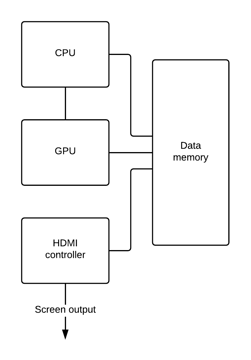
\includegraphics[width=0.65\textwidth]{../system_overview/diagrams/logical_overview.png}
	\caption{Logical overview of the system.}
	\label{fig:logical_overview}
\end{figure}



\section{Programming model}
\subfile{../system_overview/programming_model}

\todo{We should explain the programming model with an easy-to follow example}
\end{document}


% CPU
\documentclass[../main/report.tex]{subfiles}
\begin{document}
\chapter{CPU}

Now that we have seen how to write code that colors the screen with a beautiful green color, 
it is time to see what is actually happening on the Demolicious System during this execution. 

Our journey starts in the main control unit of the Demolicious computer, namely the CPU, which is implemented on an EFM32GG Microcontroller.

In this chapter we will follow a kernel from load to execution and explain what happens behind the scenes on the CPU, which is the component on Demolicious that runs the C code seen in the last chapter.

\subfile{../cpu/functionality.tex}

\subfile{../cpu/bus.tex}

\subfile{../cpu/load-kernel.tex}

\subfile{../cpu/run-kernel.tex}

\subfile{../cpu/load-constant.tex}

\subsection{Summary}

We have seen how our kernel is bootstrapped and executed. 
The assembled kernel is uploaded to the GPU which is then given a command to run said kernel with one thread per pixel.


\end{document}


% GPU
\documentclass[../main/report.tex]{subfiles}
\begin{document}

\chapter{GPU}

The GPU is at the heart of the Demolicious system.
Inspired by SIMD and SIMT architecture and programming models, the GPU architecture is named 'GhettoCUDA' in honor of NVIDIAs CUDA environment.\todo{cite this}

The GhettoCUDA architecture is highly parallel, in that it allows for a great number of threads to execute in parallel on multiple streaming processors.
A thread is the unit of execution, in essence a single procedure, that when correctly parameterized by run-time values allows for the transformation of a set of input data to a graphical representation to be visualized by the HDMI module.
A simple kernel, requiring no input, might be one that for each pixel in the framebuffer stores the color red.

The main design challenge in creating a GPU-inspired system is managing to saturate the memory bus as much as possible, changing memory access patterns from clustering together in time to a more spread-out pattern.
To facilitate this, the architecture allowing for multiple threads to execute on each streaming processor core, with a staggered start.
This design decision allows for a steady stream of load/store instructions without requiring a system stall as one waits for memory requests to return.

\section{Responsibilities}

The GPU has a relatively simple job:
\begin{enumerate}
  \item
    Receive instructions and constant data from the MCU
  \item
    Receive kernel invocations from the MCU
  \item
    Write results to external SRAM
  \item
    Assert the 'computation finished' signal to the MCU
\end{enumerate}

\section{Architecture Overview}
\begin{figure}[H]
\centering
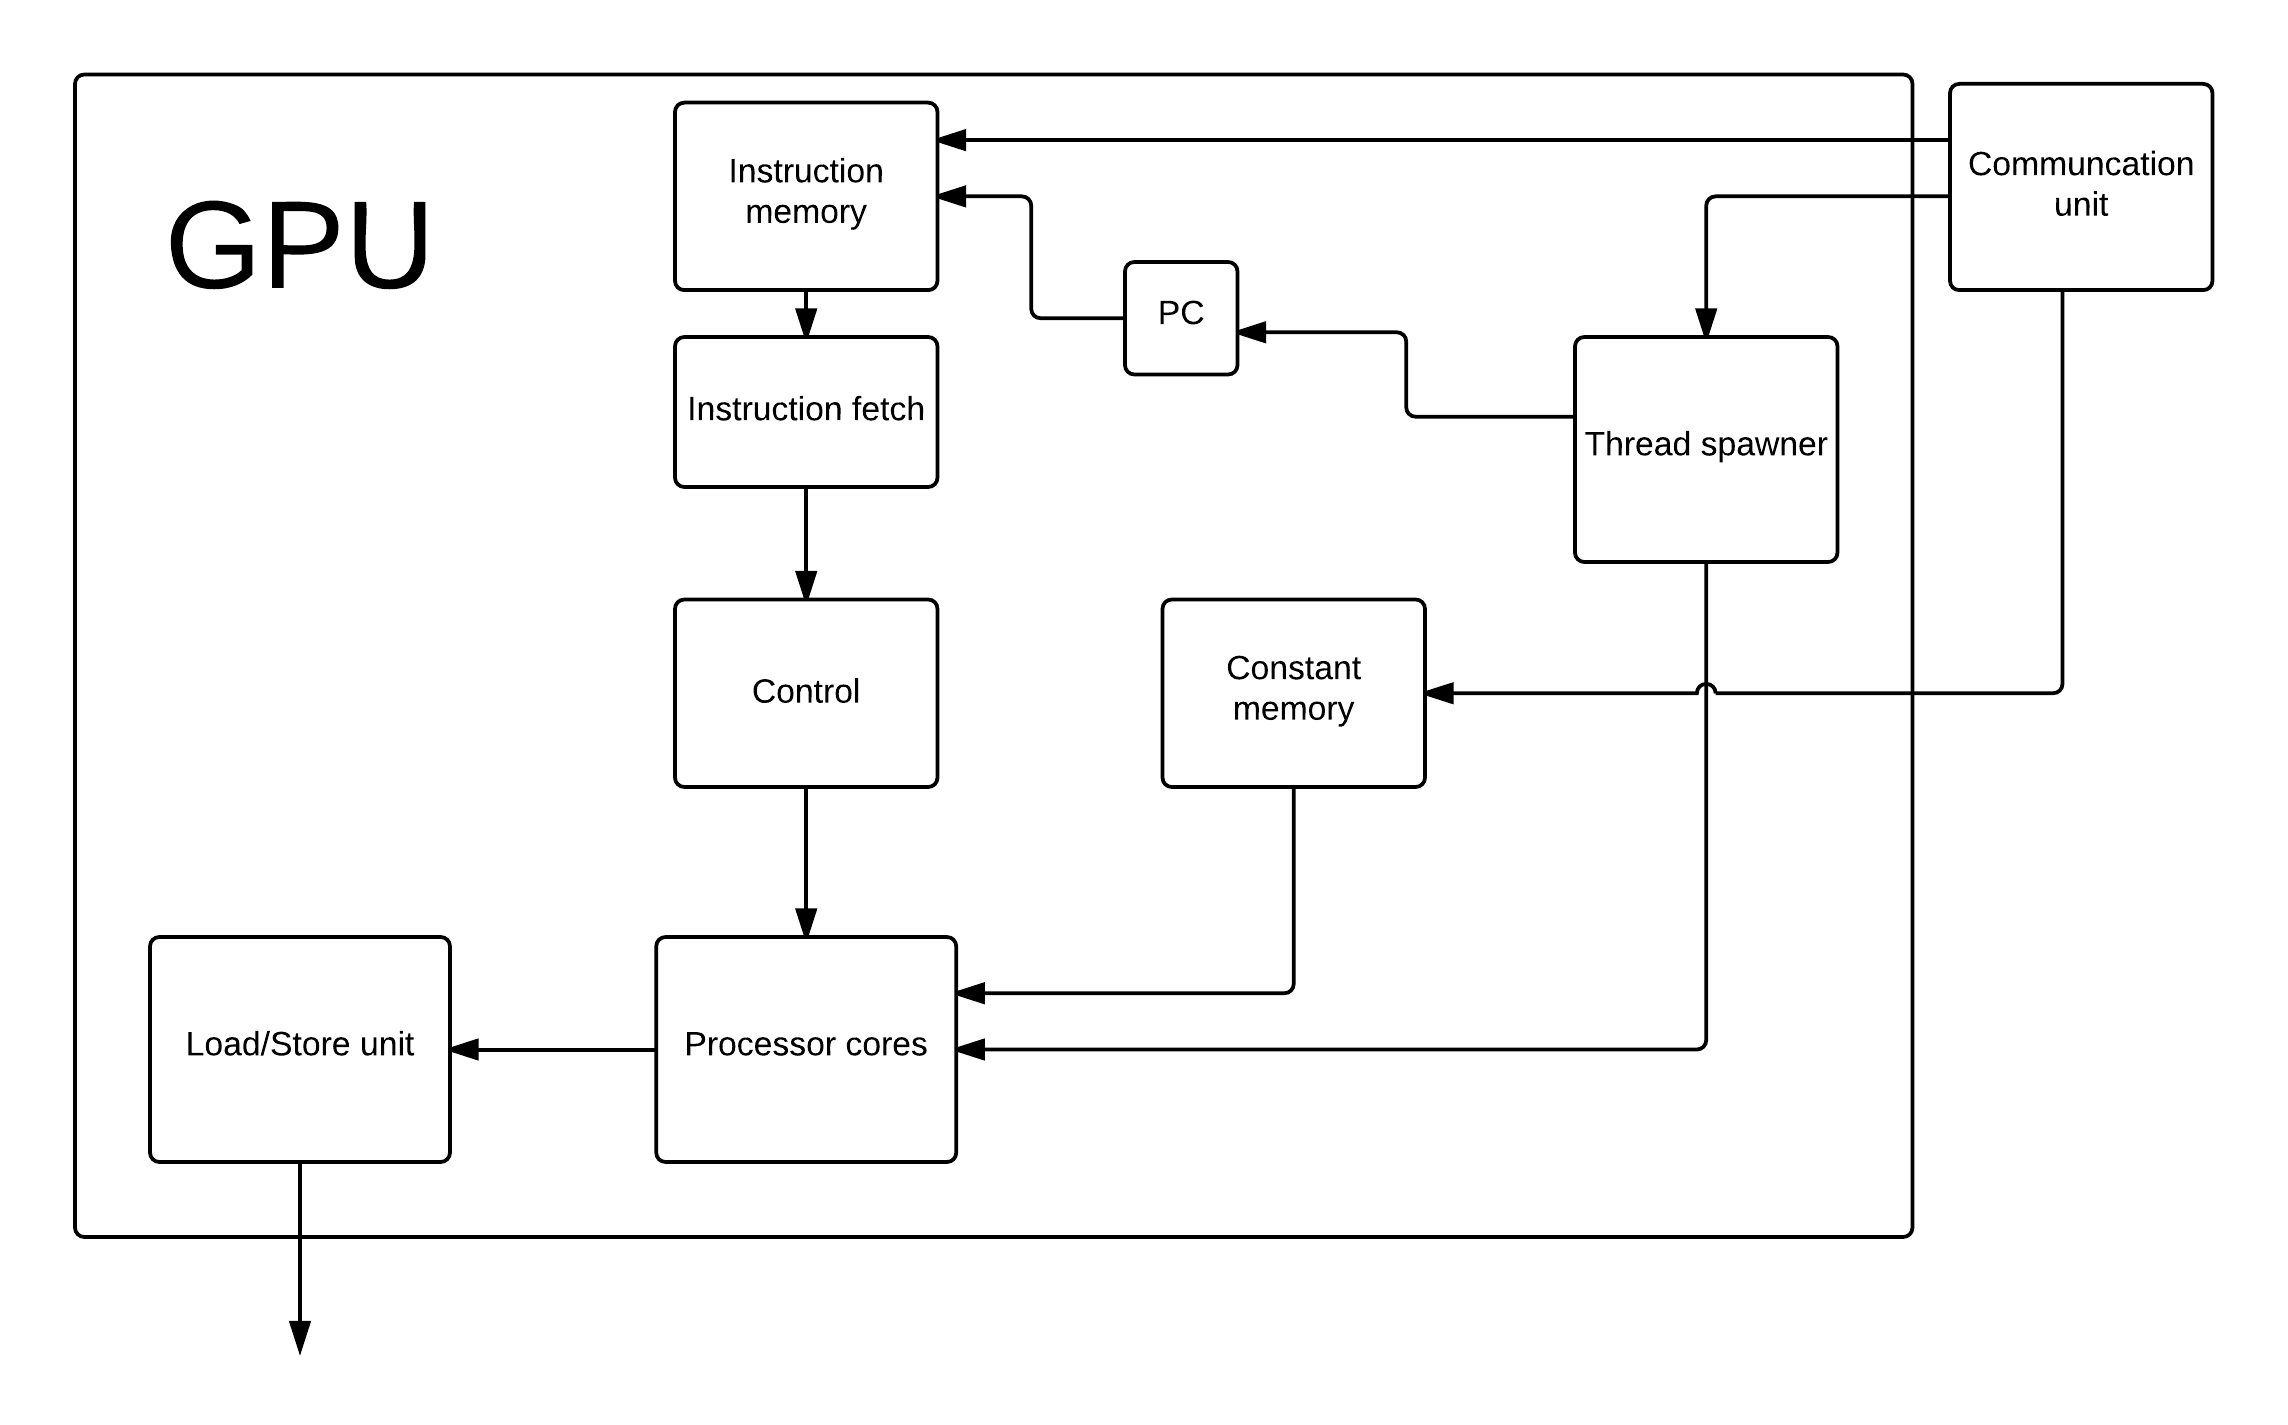
\includegraphics[width=\textwidth]{../gpu/diagrams/architecture_overview.png}
\caption{A high level overview of the GPU.}
\label{fig:architecture_overview}
\end{figure}
Figure \ref{fig:architecture_overview} presents a high level overview over the data-flow in the GPU.
The CPU issues commands to the GPU via the communication unit. Commands include actions such as launching a kernel, uploading kernels to the instruction memory, and writing to the constant memory.
Instructions are fetched from the instruction memory and decoded by the control unit, which has the responsibility of setting the control signals for the instructions.
The processors load constants from the constant memory, and uses the load/store unit for  accessing the data memory. 


\section{Kernel Structure}

\section{Receiving a Kernel Call}
\begin{figure}[H]
\centering
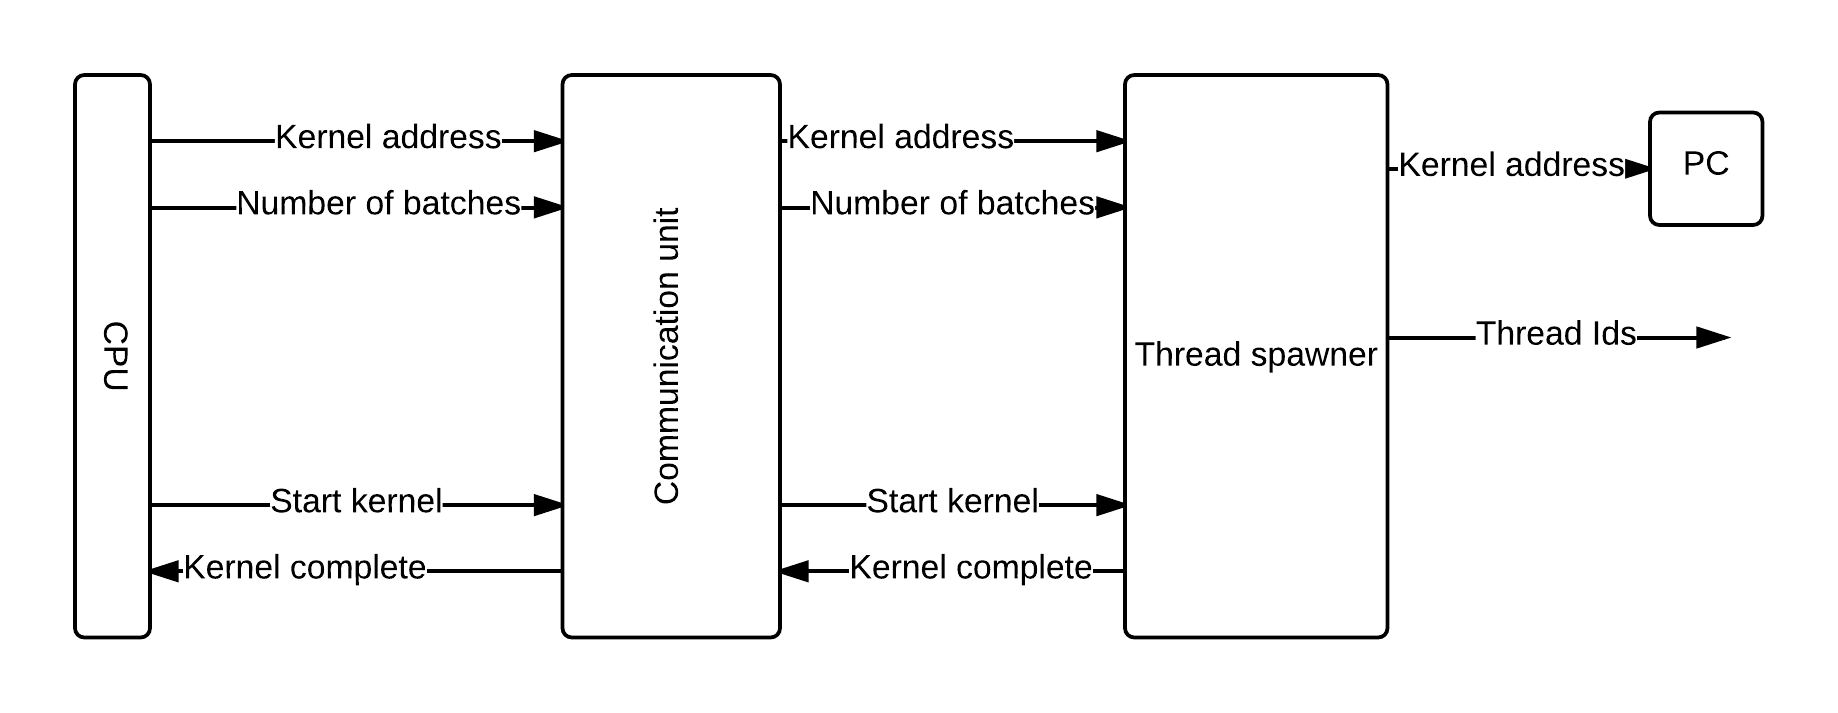
\includegraphics[width=\textwidth]{../gpu/diagrams/receiving_a_kernel_call.png}
\caption{Launching a kernel from the GPU's viewpoint.}
\label{fig:kernel_call}
\end{figure}

The communication unit is responsible for receiving kernel call requests from the CPU, and initiating the request.
A valid kernel call consists of the address of the kernel, the number of batches to launch, and asserting the launch signal.

The kernel launch signals are forwarded to the thread spawner, which writes the kernel start address to the PC register, and starts distributing threadIDs to the streaming processors. 
After holding the kernel launch signals high for one clock cycle, the communication unit has completed its role in launching the kernel.
When the kernel completes executing, the thread spawner asserts the kernel done signal, and the communication unit forwards the signal to the CPU, indicating that the kernel call has completed.


\section{Running a Kernel}
Once the thread spawner has been initiated by the communication unit, the kernel runs to completion without intervention by the CPU. 
At the beginning of a kernel run, the thread spawner assigns threadIDs to each warp in the barrel.
After the initial IDs have been assigned the GPU enters normal execution.
\begin{figure}[H]
	\centering
	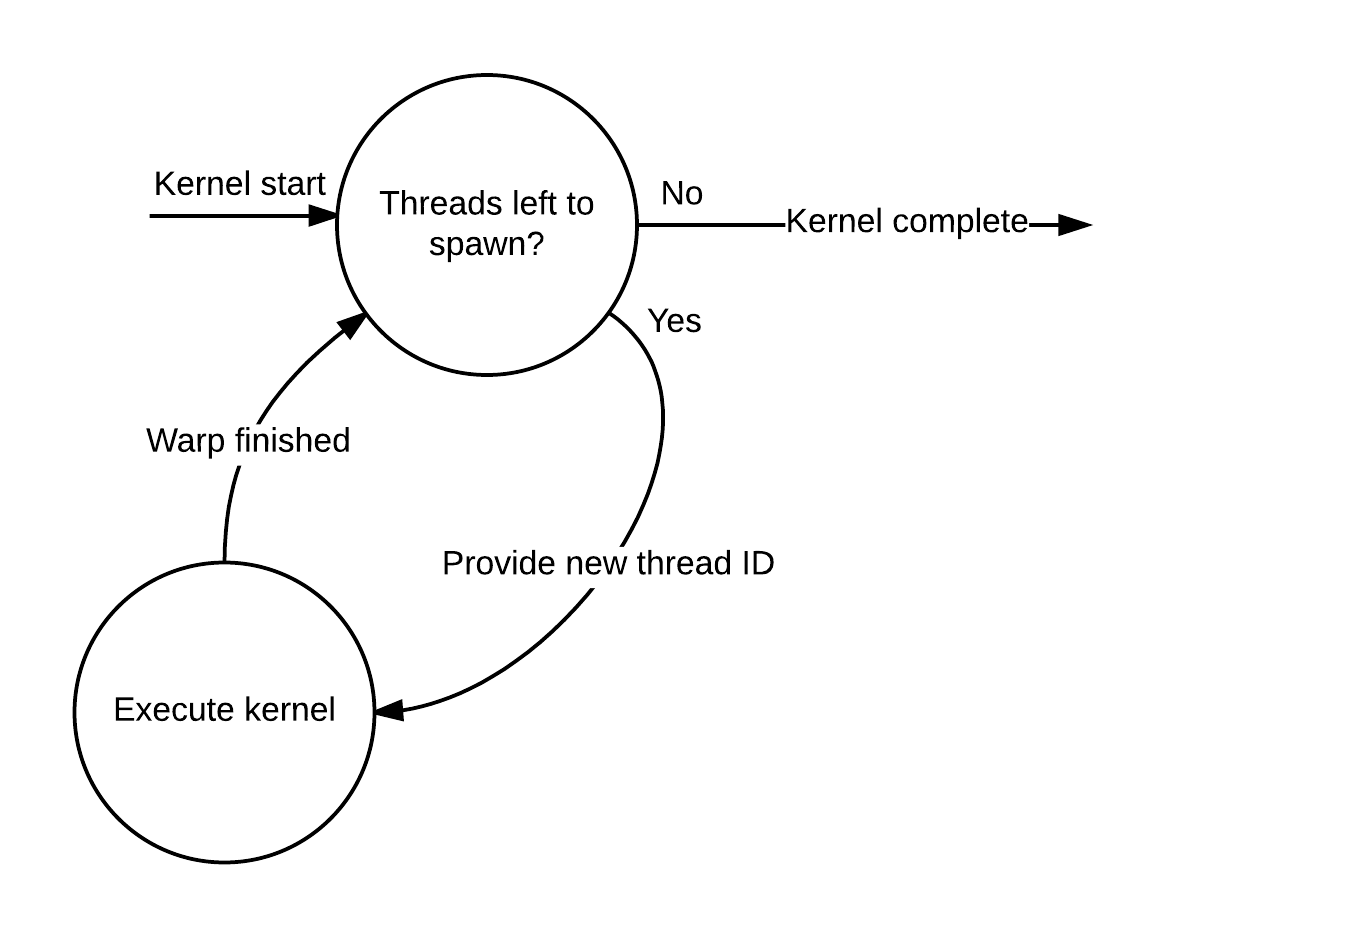
\includegraphics[width=0.9\textwidth]{../gpu/diagrams/kernel_run_state_machine.png}
	\caption{The GPU's internal state during kernel execution.}
	\label{fig:kernel_run_state_machine}
\end{figure}
A normal kernel execution can be represented by the state machine in figure \ref{fig:kernel_run_state_machine}.
During the kernel execution stage the warps execute the same instructions in lock-step one warp at a time, until the control unit encounters a \textit{Finished} instruction.
Upon receiving a \textit{Finished} instruction the control unit asserts the finished signal alerting the thread spawner that the warp requires new threadIDs.
The thread spawner keeps track of the number of threads awaiting launch.
When the thread spawner receives a \textit{Finished} instruction and no more threads are awaiting launch, the kernel run has completed.

\section{Component Details}

\todo{Can this be called something else? It's kind of confused with the component details in the PCB chapter}

\subsection{Streaming Processor}

The streaming processor is at the heart of the GhettoCUDA architecture.
A fully operational GhettoCUDA processor will have up to 32 streaming processors wired up, allowing for an extreme degree of parallelism in code execution.

The architecture of the streaming processor is inspired by the cores of the MIPS architecture.
They consist of a single ALU, a register bank, as well as logic for reading operands from thread-private registers, shared external memory and constant storage.
Each register bank is actually composed of several register files, containing a number of general- and special purpose registers.
The register bank mirrors the interface of the register file, but only exposes a single register file at a time, which one decided by the current active barrel line.
This system allows rapid context switching between the plethora of threads co-existing inside each streaming processor.

The streaming processor support conditional execution of instructions, using a dedicated mask register to decide whether instructions should be executed or not.
This allows for branch-like behavior without having to support the complex logic required for diverging threads.

When a memory request is invoked by the currently active instruction, memory addresses and data values are sampled from the currently active register file in the register directory, and passed on to the load/store unit.
Dedicated address and data store/return registers allows for simplification of both the programming model as well as requiring fewer wires between the set of streaming processors and the load/store unit.

\subsection{Thread Spawner}

The thread spawner is responsible for converting the MCUs request of n kernels executing kernel k on data set d to actual hardware threads.
As all kernels are uniquely identifiable by their respective thread ID, the thread spawner is responsible for providing strictly increasing and unique IDs.


\subsection{Register Directory}
\begin{figure}[H]
	\centering
	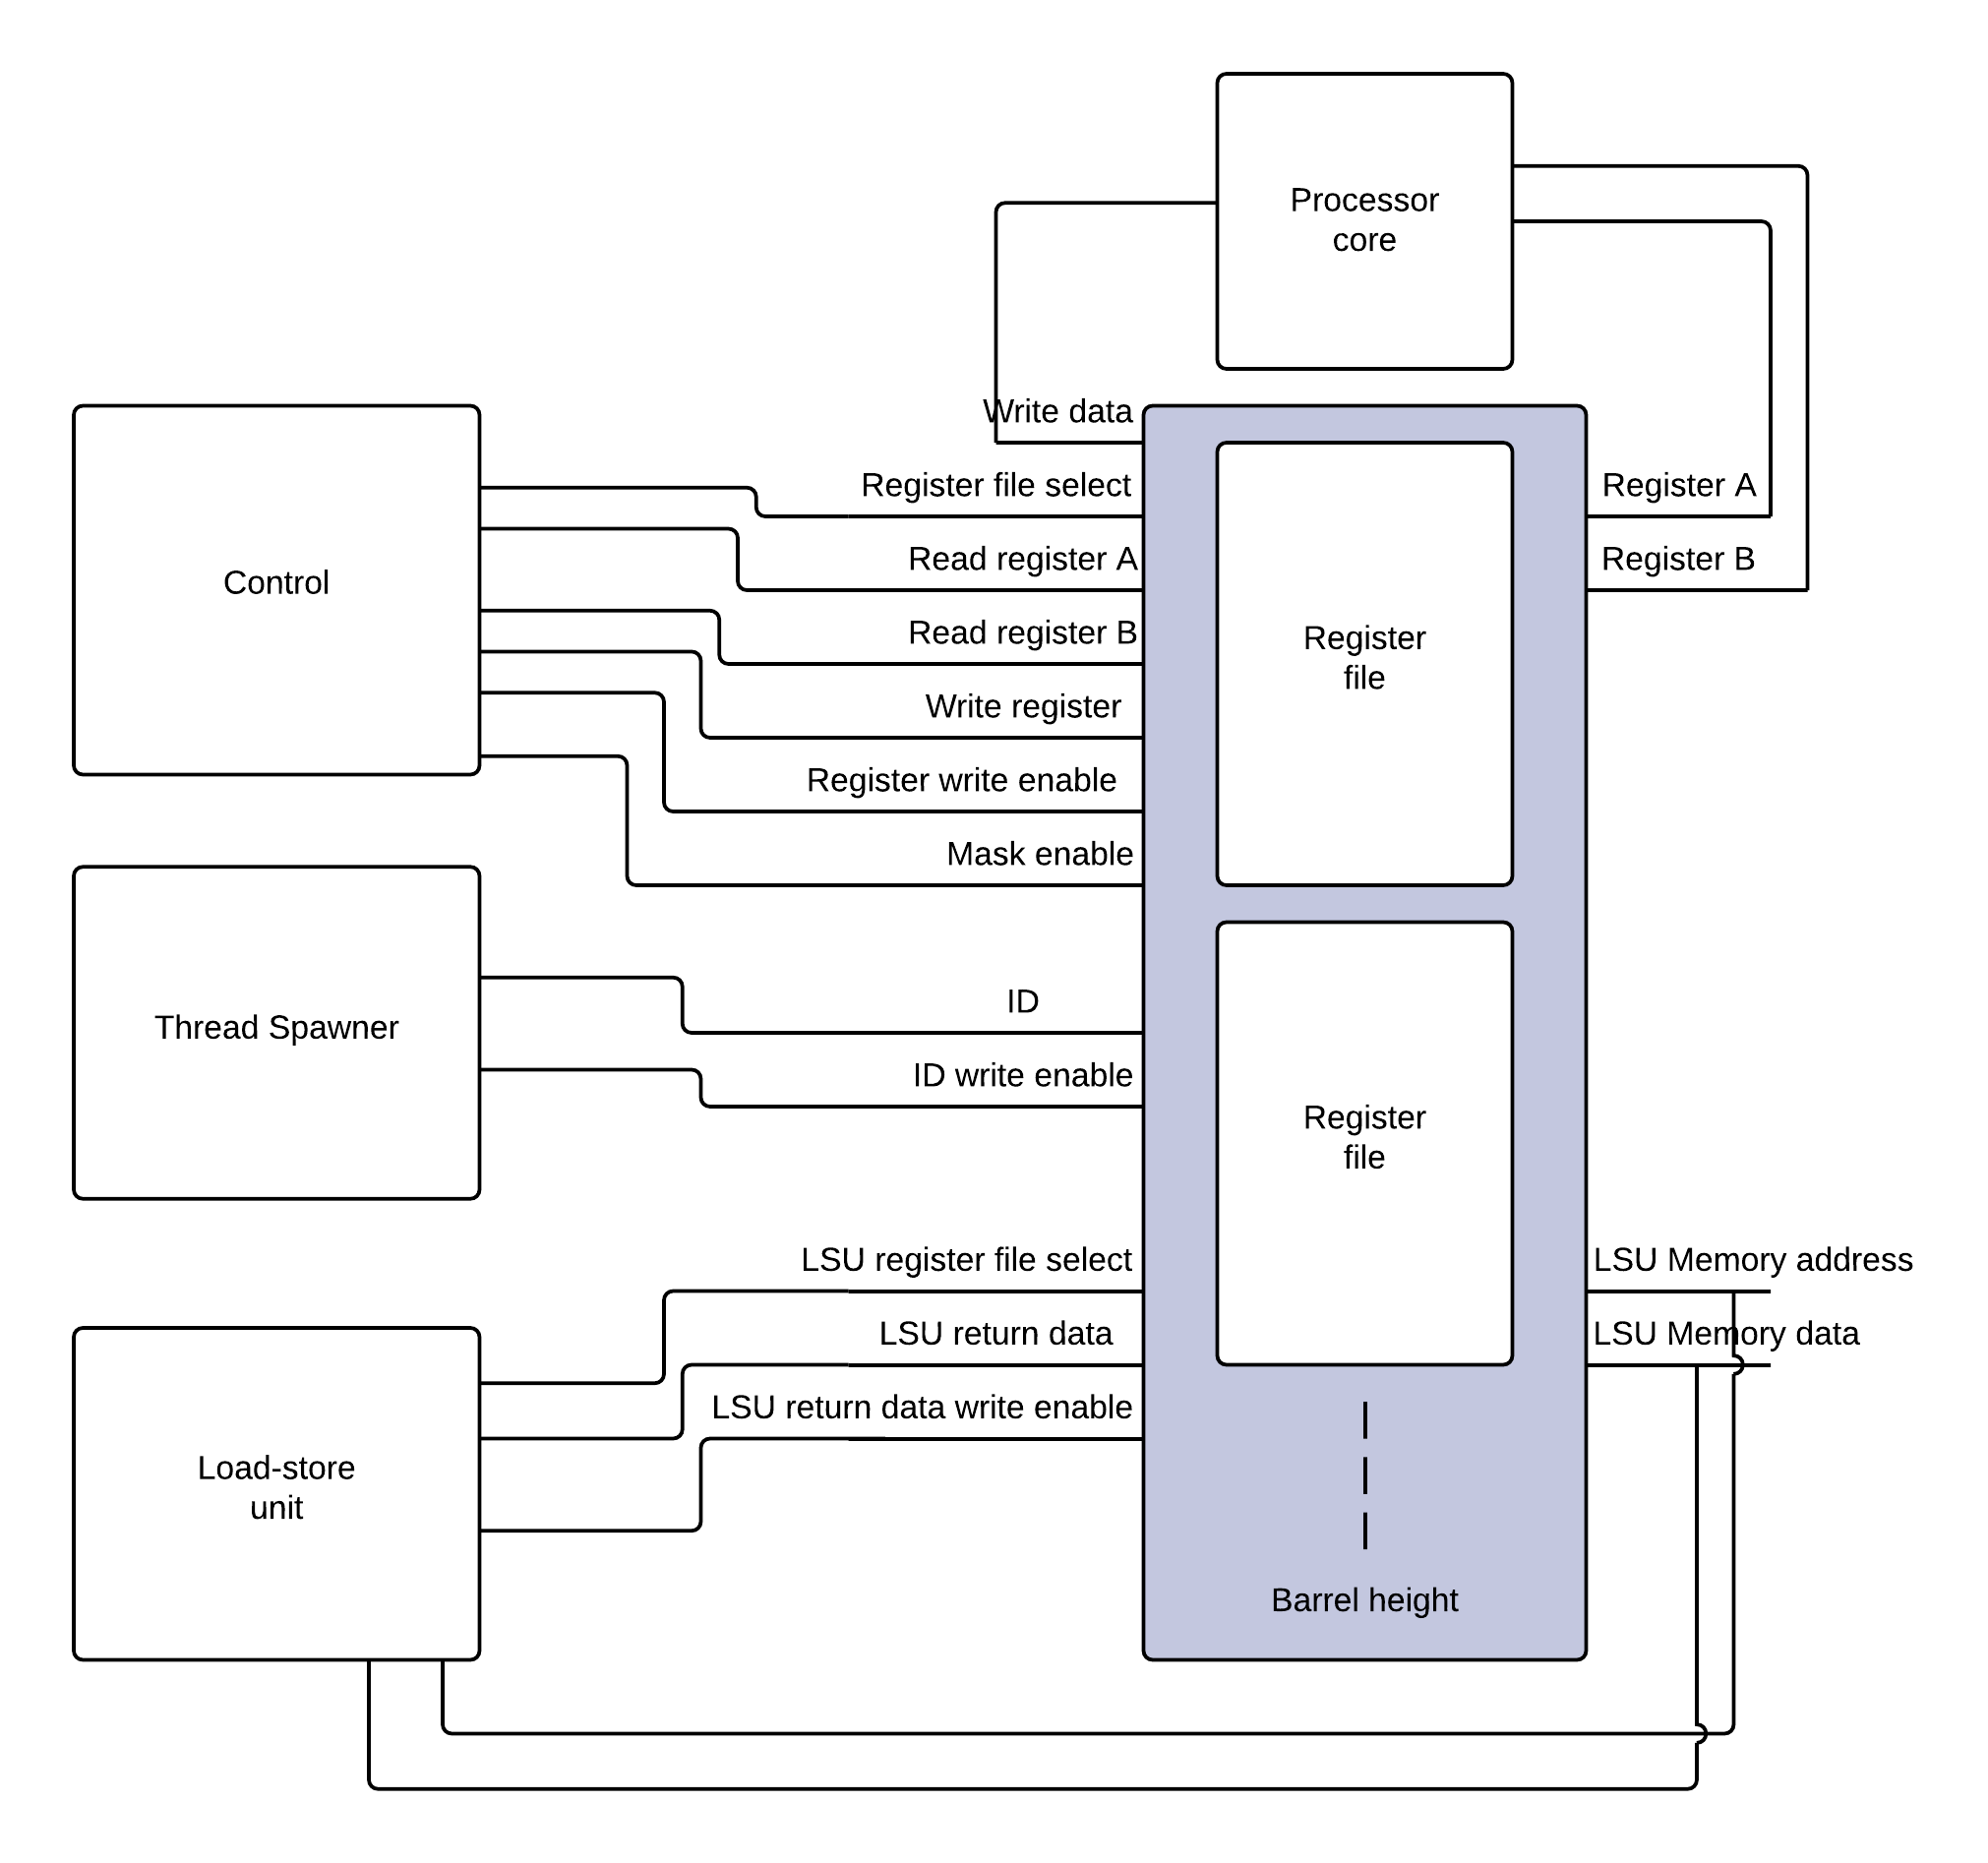
\includegraphics[width=\textwidth]{../gpu/diagrams/register_directory.png}
	\caption{The register directory, and its neighbouring components.}
	\label{fig:register_directory}
\end{figure}

There is one register directory per processor core.
Each register directory contains one register file per barrel row.
The register files include seven dedicated registers, and nine general purpose registers (Table \ref{tab:registers_overview}).

\begin{figure}[H]
	\centering
	\begin{tabular}{|c|c|c|}
		\hline Register number & Description & RW \\ 
		\hline \$0 & Zero register & Read-only \\ 
		\hline \$1 & ID High & Read/Write \\ 
		\hline \$2 & ID Low & Read/Write \\ 
		\hline \$3 & Address High & Read/Write \\ 
		\hline \$4 & Address Low & Read/Write \\ 
		\hline \$5 & LSU data & Read/Write \\ 
		\hline \$6 & Masking register & Write-only \\ 
		\hline \$7 - \$15 & General purpose registers & Read/Write \\ 
		\hline 
	\end{tabular} 
	\caption{The registers contained within the register files.}
	\label{tab:registers_overview}
\end{figure}

Individual register files are selected by using the \emph{register file select} signal.
The register file select signal is set by the control unit.
Within the register directory, the other input signals are routed to the selected register file using the select signal.
Consequently, from the processor core's point of view, there's just one register file.

The dedicated registers serve special purposes in the architecture.
Other components need to access the register files, often at the same time as the processor core is accessing another register file. 
To solve this, the special registers are given dedicated signals the other components use for reading/writing to the register file.
Ignoring registers \$0 and \$6, the rest of the dedicated registers may be used as general purpose registers.
Using them at the same time as other components are accessing them is undefined behaviour, and left as a responsibility for the programmer.

The masking register is used to enable conditional execution.
If masking is enabled the first bit of masking register is used to disable writes to the register file, making the instruction have no effect (Figure \ref{fig:masking}).
\begin{figure}[H]
	\centering
	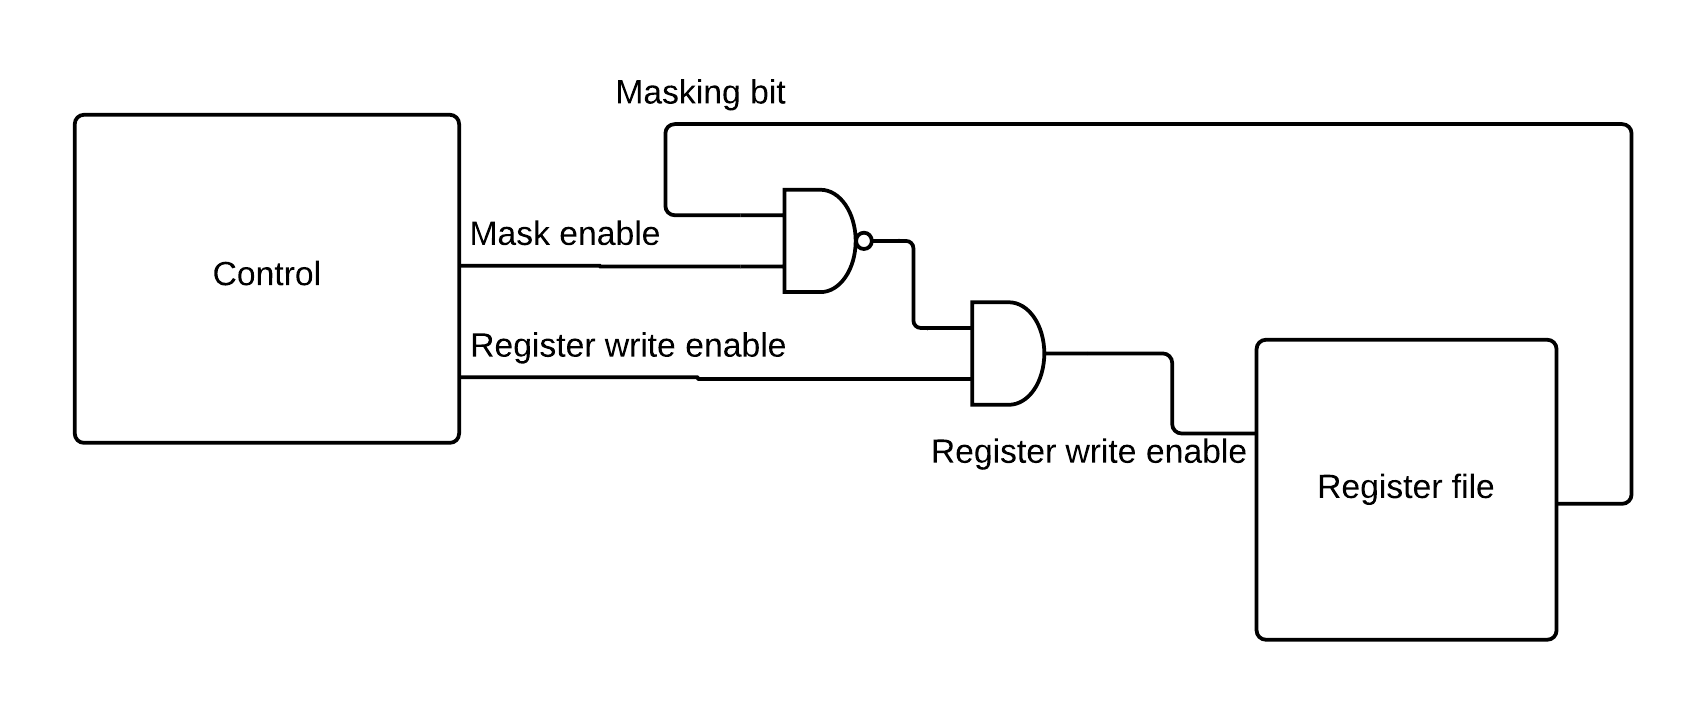
\includegraphics[width=0.8\textwidth]{../gpu/diagrams/masking.png}
	\caption{Using the mask bit to disable register writes.}
	\label{fig:masking}
\end{figure}

Data memory addresses are 20 bit wide, and thread IDs are 19 bit wide.
Registers can only store 16 bit values.	
To represent these values they are split into registers which contain the higher and lower bits.

The load store unit (LSU) has a separate signal for selecting register files.
Using the signal the LSU can write data loaded from memory into the register files on its own.


\subsection{Load/Store Unit}

\end{document}


% Comm
\documentclass[../main/report.tex]{subfiles}
\begin{document}

\chapter{On-Chip Communication Modules}

\section{Communication Unit}

\section{HDMI Unit}

\section{SRAM Arbiter}

\end{document}

%PCB
\chapter{PCB}
\label{sec:pcb}

This chapter will describe the PCB layout, the main components and the design philosophy that went into solving the system requirements.
%\section{Layout Overview}


\section{Design for Redundancy}

When designing a pcb for a system, there is no easy way to correct mistakes.
A wire can not be rerouted if there is a problem.
Becayse of this, a lot of effort has gone into making backup plans if something fails.
Each part of the pcb needs to be able to work without the rest of the pcb.
This is done by having jumpers on each section, which can be rerouted manually.
That way each part can be connected to other parts of the board, or to other sources.
Because of this, the board is not optimized for size, but was rather made to optimize for highest possible chance of success.

This small graphics explains the design philosophy of the pcb
\begin{verbatim}
     -----------------
    | Backup solution |
    |                 |
    |  -------------  |
    | | Core design | |
    | |             | |
    | |             | |
    | --------------- |
    |                 |
     -----------------
\end{verbatim}

\section{Main Components}

\subsection{Microcontroller / System Control Unit}
The EFM32 Giant Gecko 32-bit Microcontroller from Energy Micro was chosen as the controller for this project.
A microcontroller from Energy Micro was required for the task and this particular controller is
very energy efficient, which is a plus.
In addition to this, there were a lot of development boards available,
plus over half of the group had experience with this controller from the subject
TDT4258 Energy Efficient Computer Systems.

The EFM32GG990F512-BGA112 was chosen as a powerful enough version of the microcontroller.

\subsection{FPGA}
The Spartan-6 FPGA from Xilinx was chosen as the FPGA.
This particular FPGA has been used for different tasks on the university before, and the support systems are therefor available to us.
The XC6SLX45-2CSG324I version was the one used on the PCB.
A weaker version of this is avaibale for testing on development boards in the lab.

\section{Input}

The main source of data communication between microcontroller and a host PC is USB.
This protocol has been used for years on projects like these, with good results. \todo{citation needed}
Also, the power uses usb, so the protocol is already a part of the PCB.

However, if the usb fails, there are backup plans.
Primarily a serial port (RS-232) has been included to work if the USB should fail.
If this also fails, the wires from the serial port is put on headers, which can be used as GPIO pins.

\section{Output}
The main source of output from the FPGA is a HDMI connector.
This has never been done before in this projects throughout the years.

Because of this new challange, a lot of backup schemes were put in place.
The HDMI connector is put on headers, in case the connector fails.
A separate VGA module is connected to the FPGA, in case the HDMI doesn't work.
If this fails a VGA module is also connected to the microcontroller.

All of this should make sure we should be able to drive output from our pcb.

\section{Power}
USB connection with successive headers that allow for using an external power supply in case power fails.

\section{Bus}
Standard EBI connection between FPGA and MCU, but with headers in between such that external connection can be done in case of failure on one side of the connection, as well as an easy way to check transmitted signals during debugging.

\section{Clocks}
FPGA oscillator along with header on which an external oscillator resource can be connected by way of backup.
The microcontroller clocks on the other hand have a backup solution in that the microcontroller has internal RC-oscillators for use in case the crystals malfunction.

\section{Soldering}

\begin{table}
%\centering
\begin{tabular}{| L{1cm} | L{3cm} | L{3cm} | L{3cm} | L{3cm} |}
\hline
\multicolumn{5}{|c|}{Solder and test plan} \\
\hline 
Step & components & Desription & Expected results & Actual result \\\hline
5V power & usb connector & Measure voltage on the header & Measure 5 volts on the incoming power line & \\
\hline
 & & & &\\
3.3V & 3.3V header, 3.3V LDO, voltage regulator capacitors, power indicator LED and ARM programming header  & Solder the component and Messure the voltage on voltage-pin and observe teh D2 LED & Expect the power indicator LED to light up, the 3.3v power pin charged with 3.3v & \\
\hline
 & & & &\\
1.2V & 1.2V LDO, power indicator LED, voltage regulator capacitor, voltage regulator resistor. & Solder component and and messure the connector in BGA for 1.2V and observe the D1 LED & 1.2V on one connector in BGA, power indicator LED light up &\\
\hline
 & & & &\\
 BGA & EFM32GG990, LX45 & place the component on a new PCB and bake them in the oven & &\\
 \hline
 & & & &\\
 Resolder electrical circiut & power supply and LDO voltage regulator & Reconnect the electriical circuit on the new board & &\\


\end{tabular}
\caption{\label{tab:widgets}Solder plan.}
\end{table}




\end{document}

\section{Footprints}
Predominantly SMDs(surface mounted device) large enough for humans to solder(with a couple of exceptions)

\documentclass[../main/report.tex]{subfiles}
\begin{document}

\subsection{HDMI}

From a demo makers perspective, a GPU without a video output is commonly known as a space heater.
Demolicious uses HDMI for its video output, making it easy to connect to any recent video display.

HDMI is a streaming protocol; the receiver reads data from the cable at a fixed rate.
In Demolicious, the GPU has priority access to the memory.
This means that the video unit may not have access to the framebuffer (which lies in memory) when it's time to send a pixel.
To alleviate this issue, as much of the framebuffer as possible is prefetched into a buffer whenever memory is idle.
Should the buffer underflow, sending of late pixels must be abandoned.
Otherwise, pixels will not be synchronized with the position they should appear at on the screen.

Control signals assert where in the data stream a new frame of video starts and ends.
These allow the receiver to determine the resolution and refresh rate of the video.

The lowest resolution supported by HDMI is 640x480.
As this is larger than our framebuffers (64 x 64 pixels), a letterbox is added around the picture.
For debugging purposes, the letterbox consists of a low-contrast checker pattern.

To actually send the data over HDMI, control signals and pixel data are split into three channels.
They are then encoded using a scheme known as TMDS.
The purpose of TMDS is to minimize the effect of noise over the physical connection.

TMDS uses 10 bits to encode either an 8-bit color value when sending a image, or control values when not.
Demolicious uses a 16-bit word size, so colors are represented with 5 bits for red, 6 for green and 5 for blue.
These are resized to 8-bit values using a scheme that allows for both complete black and white colors.
Each channel is then serialized before being output together with a clock using differential-signaling.

Finally, to avoid a visual artifact known as \emph{screen tearing}, a technique known as \emph{V-sync} with \emph{double buffering} is used.
These techniques ensure that only complete frames of video are output, increasing visual fidelity.

\end{document}


\todo{...Uncertain ie om at vi endra litt på en del footprints, men pga hvordan fysiske komponenter funker,}

\subsubsection{Prebundled}

\subsubsection{Handmade}
Some footprints we had to make ourselves.
This was done inside Altium.
The specification for the footprints was found in the datasheets of the component in question.

When making the handmade footprints some other thoughts were taken into account.

\begin{itemize}
    \item We need to solder these components
    \item The connection on the components is physical, as long as it leads current, it will work.
    \item Some datasheets didn't match the component exactly, but was for a sister component
\end{itemize}

With this in mind we made footprints which was slightly bigger than it needed to.

\begin{verbatim}
Needed:                 Actual:
--------------          --------------
|            |          |            |
|--|      |--|       |--|--|      |--|--|
|  |      |  |       |  |  |      |  |  |
|..|      |--|       |--|..|      |--|--|
|            |          |            |
--------------          --------------
\end{verbatim}
>>>>>>> Add intro footprint


\part{Results \& Discussion}

% TESTING
\documentclass[../main/report.tex]{subfiles}
\begin{document}

\chapter{Testing}

Does it work?


\section{Component testing}
The system consists of a number of fairly isolated components.
It's valuable to test the components in isolation before they are connected.
Both implementation errors, and design flaws, can be uncovered before the components are introduced to the system.
The unit tests were implemented as VHDL test benches
Table \ref{tab:vhdl_unit_tests} describes the unit tests that were run.
\begin{table}[H]
	\centering
	\begin{tabularx}{\textwidth}{|c|X|c|}
	        \multicolumn{1}{l}{\scriptsize COMPONENT} &
	        \multicolumn{1}{l}{\scriptsize WHAT} &
	        \multicolumn{1}{l}{\scriptsize STATUS} \\
	\hline  \multirow{3}{*}{Barrel selector} 		  & Barrel row is incremented each clock cycle.  & \multirow{3}{*}{ Passed } \\
	 										 		  & Barrel row wraps around to 0. & \\			
	 										 		  & PC write enabled high on row 0.& \\								
	\hline  \multirow{2}{*}{Constant memory} 	      & Constants can be written.  & \multirow{2}{*}{ Passed } \\
	 										 		  & Constants can be read. & \\												
	\hline \multirow{2}{*}{Inst decode/Control unit}  & Decodes instruction types correctly. & \multirow{2}{*}{ Passed } \\
		   											  & Sets control signal values correctly. &\\
	\hline \multirow{2}{*}{Instruction memory} 		  & Instructions can be written. & \multirow{2}{*}{ Passed } \\
													  & Instructions are read from the correct address  & \\ 
	\hline \multirow{2}{*}{Instruction memory} 		  & Instructions can be written. & \multirow{2}{*}{ Passed } \\
													  & Instructions are read from the correct address.  & \\ 
	\hline \multirow{3}{*}{Register file} 		  	  & Read/write to general purpose registers. & \multirow{3}{*}{ Passed } \\
													  & Dedicated registers behave correctly.  & \\ 
													  & Does the masking bit work?  & \\ 													  
	\hline  Register directory 		 				  & Multiplexes input/output signals to the correct register file. & Passed  \\
	
	\hline \multirow{3}{*}{Processor core} 		  	  & Arithmetic operations. & \multirow{3}{*}{ Passed } \\
													  & Can mask instructions.  & \\ 
													  
	\hline \multirow{3}{*}{ALU} 		  			  & Computes arithmetic operations. & \multirow{3}{*}{ Passed } \\
													  & Can do left/right shifts.  & \\ 
													  & Performs \emph{Set if less than} correctly. &	\\								  											  
	\hline
	\end{tabularx} 
	\caption{Unit tests for components in the Demolicious system.}
	\label{tab:vhdl_unit_tests}
\end{table}
\section{VHDL system integration tests}


Before deploying to an actual FPGA, it is important to ensure correct behavior in system-level testbenches.
This testing is valuable, as if one can verify correct behavior in simulation, one has fewer potential errors when debugging the FPGA itself.

System tests for each of the major datapaths through the design have been created and run successfully.
The result of each test is verified by comparing all pixels in the framebuffer after the kernel has been run, to precomputed values in Isim.


\subsection{Memory Stores and Kernel Parameterization}

To verify that stores to memory, as well as constant memory, actually works, the kernel presented in listing \ref{lst:param-color-kernel} is used as a system test.
It has been relisted in listing \ref{lst:test-param-kernel} for convenience.
If successful, this allows for parameterizing kernel behaviour with values loaded at runtime, reducing the need for recompilation.

\begin{assembly}[caption={Kernel to test constant memory and parameterization}, label=lst:test-param-kernel]
ldc $data, 0
mv $address_lo, $id_lo
mv $address_hi, $id_hi
sw
thread_finished
\end{assembly}

Expected behavior of test:
\begin{enumerate}
  \item
    The color green should successfully be loaded from constant memory.
  \item
    It should be stored to memory.
  \item
    The screen should be filled with the color green.
\end{enumerate}

\subsubsection*{Simulation Results}

\begin{figure}[H]
  \centering
  \begin{subfigure}[b]{\textwidth}
    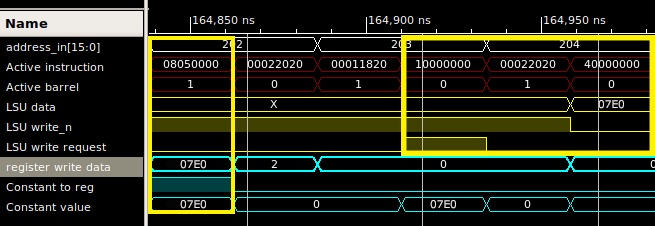
\includegraphics[width=\textwidth]{../testing/assets/Constant_load_&_store.png}
    \caption{Isim simulation showing constant load and store word}
    \label{fig:isim-kernel-parameterization}
  \end{subfigure}
  \begin{subfigure}[b]{0.3\textwidth}
    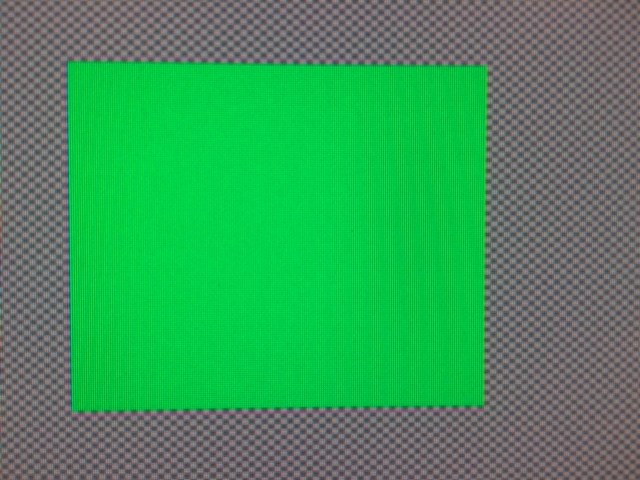
\includegraphics[width=\textwidth]{../testing/assets/green_screen.jpg}
    \caption{LX16 run}
    \label{fig:LX16-kernel-parameterization}
  \end{subfigure}
  \caption{Results from simulation and LX16 of fillscreen kernel}
\end{figure}

In the left yellow square of figure \ref{fig:isim-kernel-parameterization}, one can see the load constant instruction being executed (0x08050000) in barrel line 1.
The Constant to reg signal is asserted, and the constant value 0x07E0 is passed into the register write data signal.

In the right yellow square, the store word instruction (0x100000000) executes in barrel line 0.
The LSU accepts the write request same cycle (LSU write request goes high), and two cycles later the request packet reaches the LSU data line.
The LSU asserts LSU write\_n, (the signal is active low), and external RAM handles the store request.

The testbench passes, and values have now been successfully written to memory.
It also runs on actual hardware, the result shown in figure \ref{fig:LX16-kernel-parameterization}.

\subsection{Masked Instruction Execution}

Masked instructions are used to allow for some degree of conditional execution in the lack of proper branching and jumps.
This requires that the architecture actually respects the mask bit when set.
The masked execution kernel presented earlier in listing \ref{lst:masked-execution} is used for this test.
It has been relisted in listing \ref{lst:test-masked-execution} for convenience.

\begin{assembly}[caption=Conditional execution using predicated instructions, label=lst:test-masked-execution]
ldc $10, 0 ; Load color one
ldc $11, 1 ; Load color two
srl $mask, $id_lo, 6 ; Shift to the right converts ID to y pos
mv $data, $10
? mv $data, $11 ; Will only be executed every other row
mv $address_lo, $id_lo
mv $address_hi, $id_hi
sw
thread_finished
\end{assembly}

Expected behavior of test:
\begin{enumerate}
  \item
    Each row should be colored according to the last bit of their y position.
\end{enumerate}

\subsubsection*{Simulation Results}

\begin{figure}[H]
  \centering
  \begin{subfigure}[b]{\textwidth}
    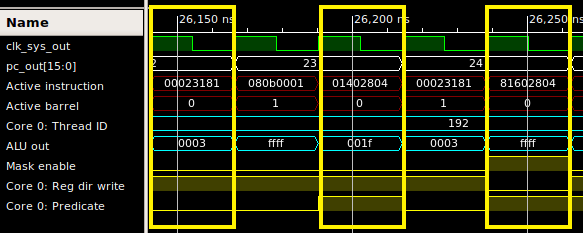
\includegraphics[width=\textwidth]{../testing/assets/masking-yes.png}
    \caption{Isim simulation showing successful masking.}
    \label{fig:isim-masked-execution}
  \end{subfigure}
  \begin{subfigure}[b]{0.3\textwidth}
    
\includegraphics[width=\textwidth]{../testing/assets/lines.jpg}
    \caption{LX16 run}
    \label{fig:LX16-masked-execution}
  \end{subfigure}
  \caption{Results from simulation and LX16 of masked execution}
\end{figure}

In the left yellow square of figure \ref{fig:isim-masked-execution}, we can see the \verb/srl/ instruction being executed (0x00023181). As this thread has thread id 192, the result out is 3.
The low bit is stored into the mask register, enabling masking for this thread.

In the middle yellow square, barrel 0 is once again active, and we can see that the predicate bit of core 0 has been asserted.
As this instruction isn't masked, the predicate bit is ignored and the value of 001f is stored into the data register.

In the right yellow square, the conditional data move is executed (0x81602804).
As the mask enable signal goes high, the register write enable signal is pulled low due to the predicate bit, resulting in the data not being written to registers.

The testbench passes, and predicated instructions are not executed when masking is enabled.
As can be seen in figure \ref{fig:LX16-masked-execution}, the kernel runs on actual hardware, and every second line is colored differently.


\subsection{Loads from Primary Memory}

If one wishes to support multi-pass kernels, that is a kernel that uses the result of previous kernels to compute its own result, then results have to be stored and loaded from somewhere persistent.
Stores to main memory have already been confirmed working, so load instructions are up next for testing.
With functioning loads, it is fairly straightforward to implement things like Conway's Game of Life  \cite{game-of-life} for the Demolicious system.

The fillscreen kernel from earlier is modified to load its value from main memory, and store it back to the framebuffer.
It is presented in figure \ref{lst:test-load-kernel}.

\begin{assembly}[caption={Kernel to test loads from main memory}, label=lst:test-load-kernel]
mv $address_hi, $0         ; Load some color from main memory
mv $address_lo, $0
lw
mv $address_hi, $id_hi
ldi $8, 2
add $address_lo, $8, $id_lo
sw                         ; Store data to ID + 2, to avoid overriding address 0
nop
thread_finished
\end{assembly}

Expected behavior of test:
\begin{enumerate}
  \item
    The loaded color should be stored to the entire framebuffer
\end{enumerate}

\subsubsection*{Simulation Results}

\begin{figure}[H]
  \centering
  \begin{subfigure}[b]{\textwidth}
    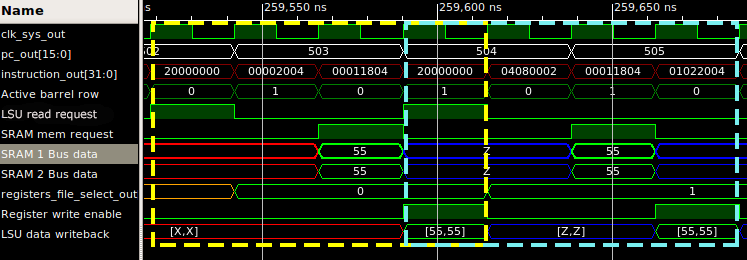
\includegraphics[width=\textwidth]{../testing/assets/Load-Store-working.png}
    \caption{Isim simulation showing working loads from memory}
    \label{fig:isim-load-kernel}
  \end{subfigure}
  \begin{subfigure}[b]{0.3\textwidth}
    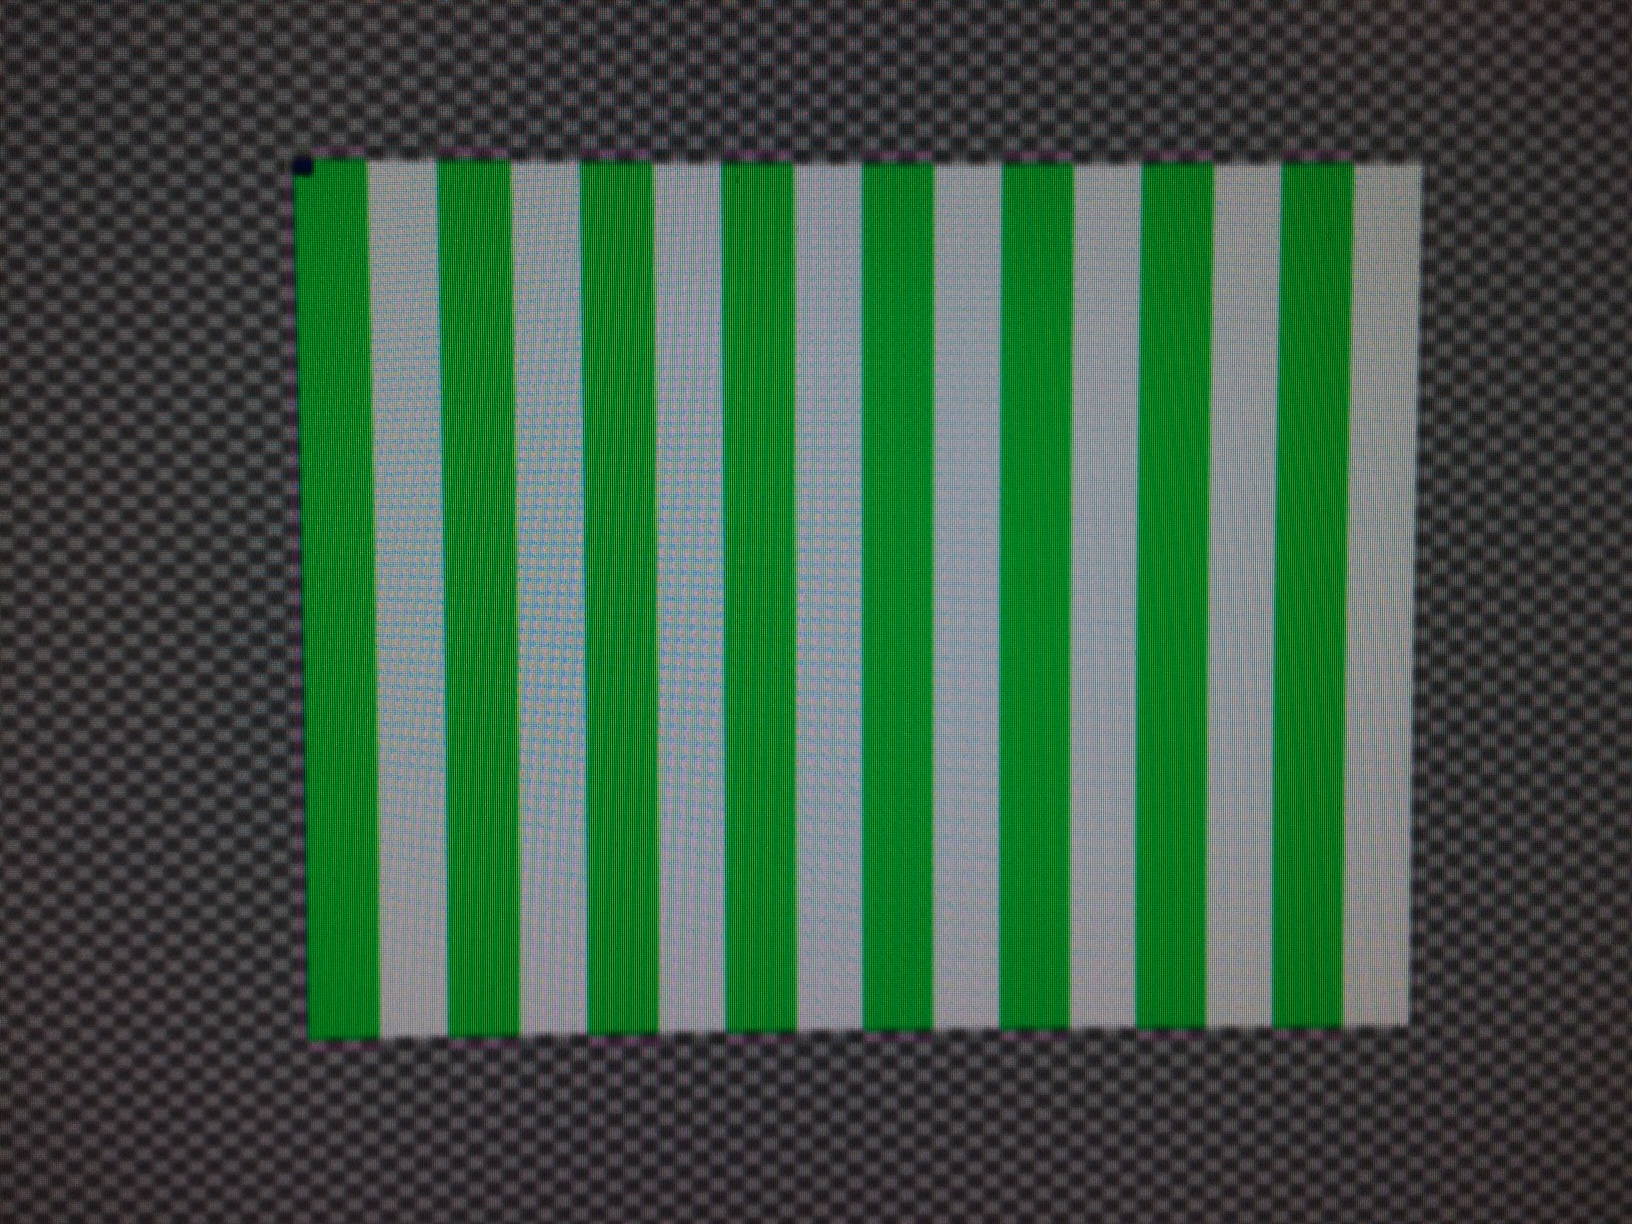
\includegraphics[width=\textwidth]{../testing/assets/halfworking-load.jpg}
    \caption{LX16 run}
    \label{fig:LX16-load-kernel}
  \end{subfigure}
  \caption{Results from simulation and LX16 of load kernel}
\end{figure}

Figure \ref{fig:isim-load-kernel} shows a barrel of height 2 performing successful loads.

In the first cycle of the yellow dotted square, barrel row 0 executes a load word instruction (0x20000000).
LSU read request is asserted in the control, and routed to the LSU.
Two cycles later the request has passed through the LSU unit, and SRAM responds with the value 55.
In the last cycle of the yellow square, the LSU asynchronously writes the result back to the registers storing the values on the LSU data writeback line to barrel row 0.

In the blue dotted square, the same procedure is executed again, this time for the second barrel row.
Notice that register\_file\_select is now set to 1, writing the result back to the second barrel row.

The testbench passes. Multi-pass kernels can now successfully be implemented.

There is however a discrepancy between the simulation and the actual implementation, resulting in the LSU dropping some writebacks, as shown in figure \ref{fig:LX16-load-kernel}.
Both the RAM used for simulation, as well as the SRAM located on the PCB is combinatoric.
On the development kit however, SRAM had to be mapped onto block RAM due to a lack of space.
This forces the RAM to be clock driven, not allowing for the same-cycle memory responses required, and therefore dropping writebacks.

\subfile{../testing/io_testing.tex}

\subfile{../testing/pcb-testing.tex}

\end{document}


% RESULTS
\documentclass[../main/report.tex]{subfiles}
\begin{document}

\chapter{Results}

\section{Scalability of the Demolicious system}
\label{sec:scalability}

The architecture of the Demolicious system easily scales to a larger number of processors.
As there is a linear relationship between the number of streaming processors on chip and processor throughput, one can simply add more cores to increase performance.

Limiting factors to this scalability include:
\begin{enumerate}
  \item
    The more cores, the lower the clock frequency, as signal propagation time and fanout increases
  \item
    Space available on the chosen FPGA
  \item
    Power consumption constraints, as more cores increase active power consumption
\end{enumerate}

%LX45 usage
%
%8% lut, 1% slice
%
%12% lut, 2%slice fanout 4.57, 3.631 lut flipflop pairs
%
%
%28% LUT, 5% slice 8393 lut flip flop pairs
%
%
%6% Slice, 25% LUT, 36% occupied, 7958 lut flip flop pairs
%
%Not synthesizable

\todo{These numbers need regenerating. I'll do it tomorrow}
\begin{table}[H]
\begin{tabularx}{\textwidth}{cccccc}
\hline
Cores & Crit. path & Max freq. & Dynamic + quiescent power & LX16 & LX45 \\
\hline
\hline
2 / 2      & 17.103ns      & 58.469MHz & 0.272 W: 0.088 W + 0.184 W & \checkmark & \checkmark  \\
4 / 2     & 17.959ns      & 55.682MHz & 0.292 W: 0.107 W + 0.184 W & \checkmark & \checkmark \\
8 / 4   & 19.722ns      & 50.108MHz & 0.353 W: 0.168 W + 0.186 W &            & \checkmark \\
16 / 8     & X  & X & X          & \\
       &               &           &                   &    & \\
\hline
\end{tabularx}
\caption{Hardware configurations compared. Harvested from post place \& route static simulation.}
\label{table:scalability}
\end{table}

The 4-core design fits with room to spare on the LX16, but does not fit the 8-core design.
The LX45 shifts this up one notch, fitting the 8-core design, but being unable to place \& route the 16-core design.
For all processor designs, the critical path passes from the immediate field of the instruction through the ALU into the active register file.
This is something that could be increased drastically by pipelining the processor.

Figure \ref{table:scalability} shows that there is a negligible drop in maximum frequency from two to eight cores.
At 50.108MHz with 8 cores, the GPU has an instruction throughput of ~400 mips.
This compares favorably to the ~117 mips of the two-core architecture.

It does however come with a 100mAh increase in power draw.
Luckily this only constitutes a 30\% total increase in power, considerably less than the fourfold improvement in GPU throughput.
The decrease in execution time will allow both the host CPU and the GPU to enter lower power states quicker, reducing static power consumption.

\section{Performance}

In the Demolicious system, the kernel calls can be issued by the CPU in only a few cycles.
This means that the number of frames per second (FPS) that the system can display is dominated by the run time of the kernels.

\begin{figure}[H]
	\centering
	\begin{subfigure}[t]{0.45\textwidth}
		\centering
		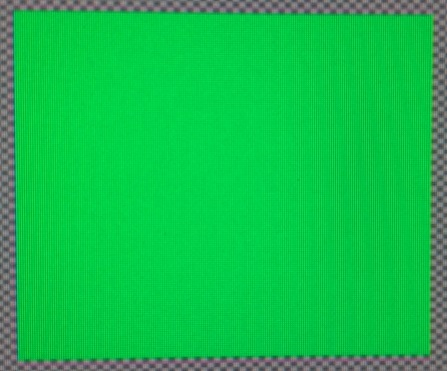
\includegraphics[width=\textwidth]{../results/diagrams/green_screen_run.jpg}
		\caption{Output from the green screen kernel.}
	\end{subfigure} 
	\begin{subfigure}[t]{0.45\textwidth}
		\centering
		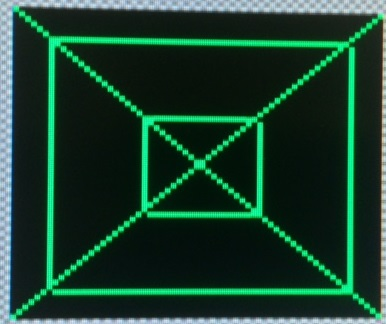
\includegraphics[width=\textwidth]{../results/diagrams/kernel_run_tunnel.jpg}	
		\caption{Output from the tunnel kernel (Listing \ref{lst:tunnel-kernel}).}
	\end{subfigure}
	\caption{Running two example kernels.}
	\label{fig:kernel_outputs}

\end{figure}

Figure \ref{fig:kernel_outputs} shows the output from the green screen kernel, and the more complex tunnel effect kernel.
It's desirable that both these kernels can be run at about 30 FPS.
Using the results presented in section \ref{sec:scalability}, the expected frames per second for varying resolutions can be estimated.

\begin{figure}[H]
	\centering
		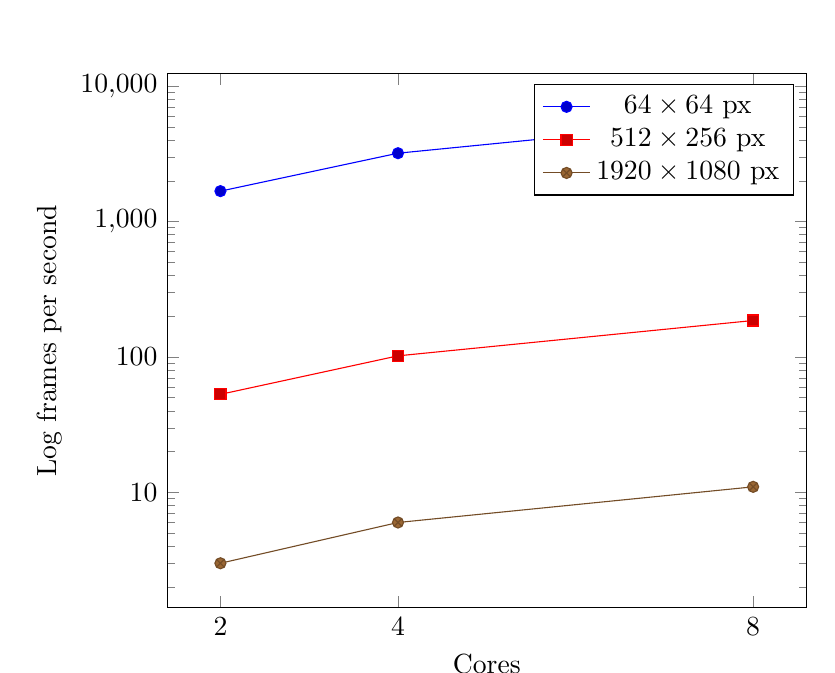
\begin{tikzpicture}
		   \begin{semilogyaxis}[
		   	   width=0.8\textwidth,
			   log ticks with fixed point,
		       xlabel=Cores,
		       ylabel=Log frames per second,
		       xtick = {2,4,8}
		   ]
				
		     \addplot plot coordinates {
		      	(2, 1678)
		      	(4, 3198)
    			(8, 5813)
		    
		  	 };
				
		   \addplot plot coordinates {
		      (2, 53)
		      (4, 102)
		      (8, 186)
		   };
		   
		   \addplot plot coordinates {
		      (2, 3)
		      (4, 6)
		      (8, 11)
		   };
		      
		   \legend{
		   $64\times64$ px \\
		   $512\times256$ px\\
		   $1920\times1080$ px\\}

		   \end{semilogyaxis}
		\end{tikzpicture}
		\caption{Running the green screen kernel.}
		\label{fig:kernel_green_screen_fps}
\end{figure}	
\begin{figure}[H]
	\centering
	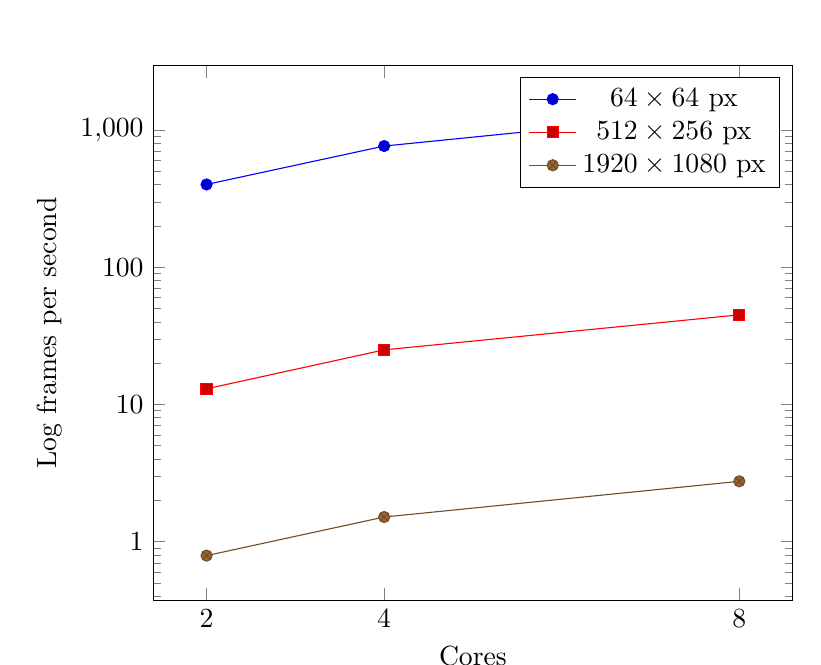
\begin{tikzpicture}
	 \begin{semilogyaxis}[
	 	 width=0.8\textwidth,
	     log ticks with fixed point,
	     xlabel=Cores,
	     ylabel=Log frames per second,
		     xtick = {2,4,8}
		 ]
		 \addplot plot coordinates {
		    (2, 402)
		    (4, 766)
		    (8, 1394)
		 };
		 \addplot plot coordinates {
		    (2, 13)
		    (4, 25 )
		    (8, 45)
		 };
		 \addplot plot coordinates {
		    (2, 0.79)
		    (4, 1.51)
		    (8, 2.75)
		 };
 
 
		 \legend{$64\times64$ px\\
		 $512\times256$ px\\
		 $1920\times1080$ px\\}

		 \end{semilogyaxis}
	\end{tikzpicture}
	\caption{Running the tunnel kernel.}	
	\label{fig:kernel_tunnel_fps}
\end{figure}


The figures \ref{fig:kernel_tunnel_fps}, and \ref{fig:kernel_green_screen_fps} display the relationship between frame rate, resolution and number of cores.
Both figures display that doubling the amount of core roughly doubles the frame rate.

For a configuration of cores, the time it takes to process one pixel is constant.
This means that the time to execute one kernel scales linearly with the resolution.
When the output resolution is increased, the amount of pixels to process increases quadratically.
As a consequence the frame rate decreases quadratically when the resolution grows.
  
For the target resolution for the project, which is $512\times256$, the project goal of maintaining 30 fps is achieved.

\section{Video output}
The Demolicious system can output to a screen using HDMI.
The minimum resolution permitted by the HDMI protocol is $640\times480$,
but the size of the data memory limits the actual resolution to $512\times256$ pixels.
The rest of the screen is padded with a checker pattern.
Most of the time the output image is correct.
However, the output image is distorted under certain conditions.
\begin{figure}[H]
	\centering
	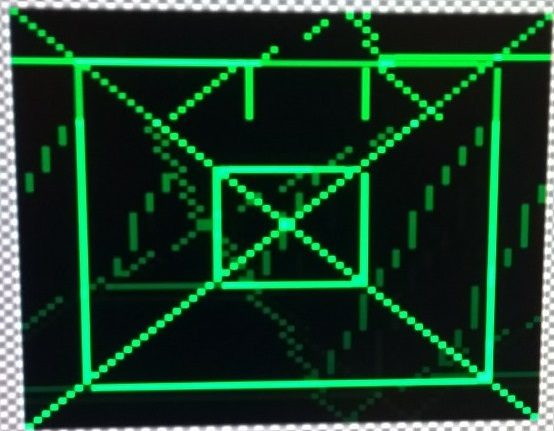
\includegraphics[width=0.8\textwidth]{../results/diagrams/flicker.jpg}
	\caption{Flickering when running the tunnel kernel. This picture was exposed over two frames.}
	\label{fig:flickering}
\end{figure}
Some kernels exhibit intermittent flickering (Figure \ref{fig:flickering}).
The exact reason for why this occurs is unclear, but
it can be observed that the flicker contains parts of the last frame. 
This may be caused by a failure in the synchronization mechanism in the video unit.

Since the GPU has priority on memory access, the video unit may get starved for data.
When the video unit is starved the buffer containing pixels to output will underflow.
For the duration of the starve, a line containing the previous pixel on the bus will be displayed on the screen.

\section{Single vs double buffering}

Screen tearing is a visual artifact where parts of two consecutive frames are displayed at the same time.
This occurs because the video unit reads the frame buffer before the GPU has finished rendering it.  
In figure \ref{fig:single_buffering} the artifact can be observed, occurrences are marked with red circles.

\begin{figure}[H]
	\centering
	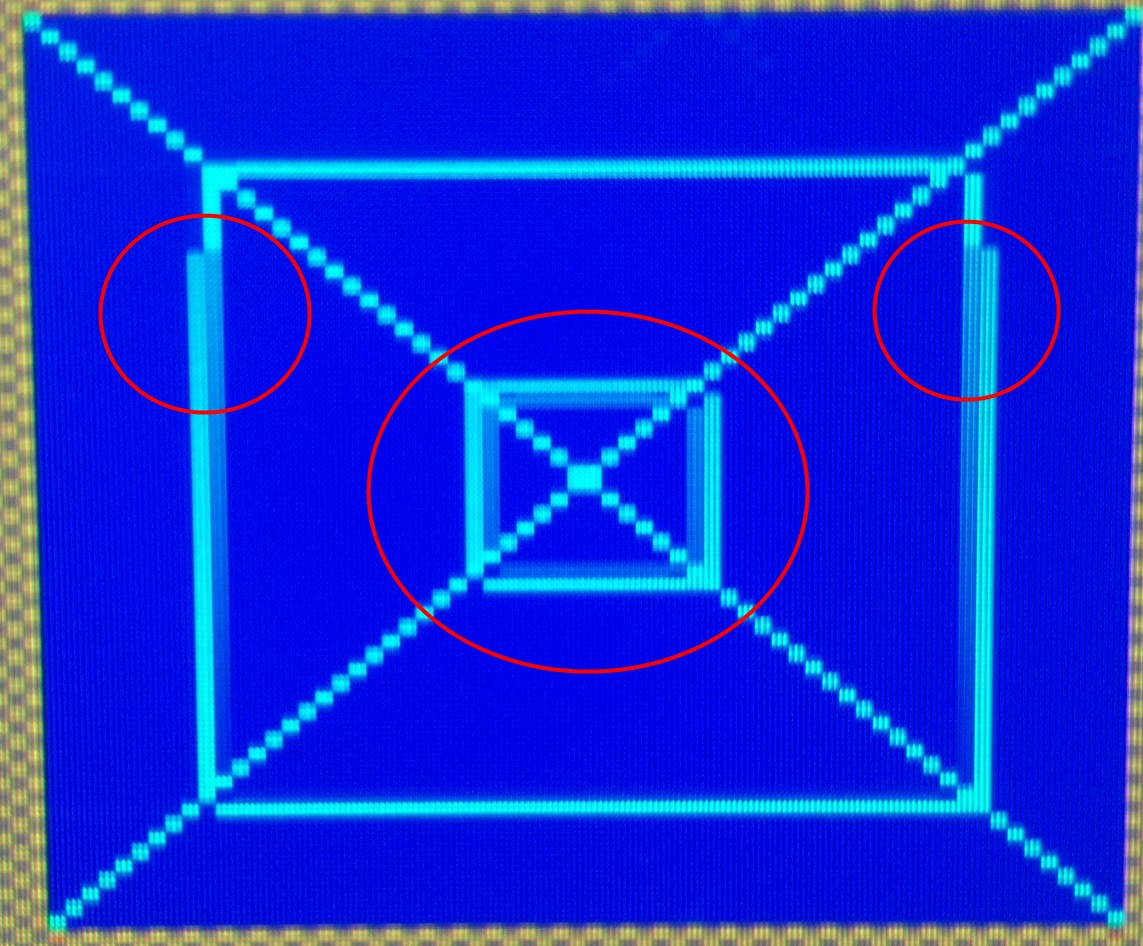
\includegraphics[width=0.5\textwidth]{diagrams/single_buffering.png}
	\caption{Single buffering.}
	\label{fig:single_buffering}
\end{figure}
Double buffering is a technique to remove this artifact.
As the name implies two independent frame buffers are used.
While one frame buffer is being read and displayed on screen, 
the next frame is rendered to an off-screen frame buffer.
Once the frame has finished rendering the frame buffers are swapped, and the frame is displayed by the video unit.
In figure \ref{fig:double_buffering} it can be observed that double buffering improves the quality of the image substantially.
The image in the figure does have some artifacts, but the ones caused by single buffering are no longer present.
\begin{figure}[H]
	\centering
	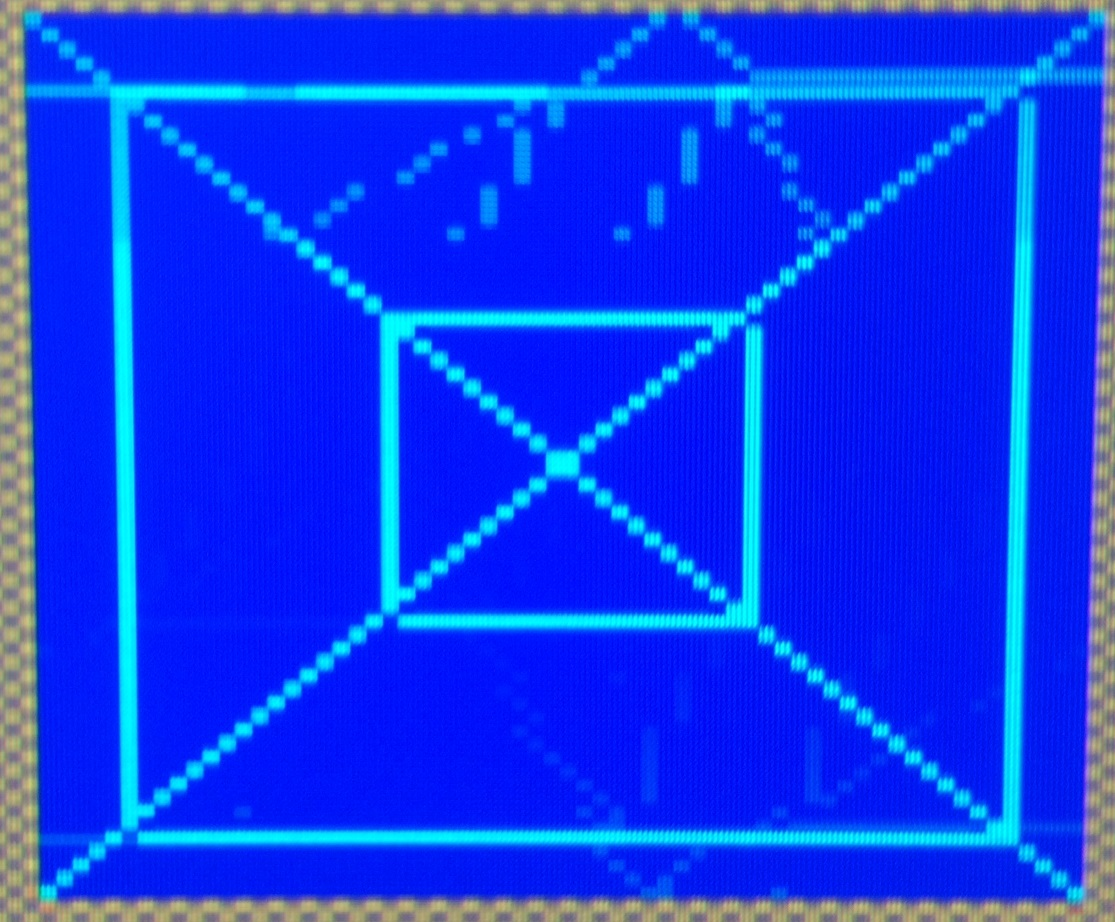
\includegraphics[width=0.5\textwidth]{diagrams/double_buffering.png}
	\caption{Double buffering.}
	\label{fig:double_buffering}
\end{figure}

\section{Power efficiency}

Demolicious has been designed with the goal \ref{tab:goals} of allowing the host system to sleep as much as possible.
Due to its computationally expensive nature, a GPU will consume a lot of power.
By quickly and efficiently executing the kernel at hand, the GPU can be put in a lower power mode, reducing static power consumption to a minimum.

With a power draw of \SI{0.353}{W} for a Demolicious setup of 8 cores \ref{table:scalability},
it is in the interest of nature to keep it spinning for as short as possible.
\todo{find number}
The EFM32GG MCU has a power draw of NUMBER in energy mode 0.
When the host program is running as an interrupt-based program instead of busy-waiting for kernel result, it may enter energy savings mode 1 or 2.
These modes introduce significant energy savings, allowing the CPU consume very little power when waiting for GPU execution to complete.

There are two use-cases resulting in different sleep times for the MCU
\begin{enumerate}
  \item
    A recurring calculation, for example rendering frames targeting 60 fps.
    The MCU will then be able to stay in deep sleep for the most of the time, waking only every 16 ms to calculate new kernel parameters, dispatching the call and going to sleep again.
  \item
    Data-throughput intensive calculation.
    Some scientific data problem requires multiple kernel passes, where a single kernel may take multiple 100 ms to complete.
    This use-case is slightly different, as one does not have a fixed interval one can wake at to check if data is finished.
    As the completion time might be somewhat variable, the MCU may go to sleep, attaching an interrupt listener on the 'kernel complete' GPIO line from the GPU.
    This allows the CPU to wait for exactly as long as is required until the kernel finishes, allowing for an extremely high sleep percentage.
\end{enumerate}

Now for some numbers!
Let's say we're targeting 30 FPS on the tunnel kernel.
The kernel itself takes 3 ms to complete, when rendered at 64 x 64 resolution.
Kernel launch overhead is negligible.
This allows the CPU to spend 90 \% of its time in EM1 or 2, netting an average of (NUMBER * 0.40 + OTHERNUMBER * 0.60) power consumption.

For the throughput-intensive kernel, say the kernel itself takes 20ms to complete.
\todo{How much time does the MCU spend executing?}
Kernel launch overhead is 5\si\micro s, resulting in a 95 \% idle time that can be spent sleeping.
This averages to a power consumption of NUMBER.


Finally, the system can run for SOME HOURS on external batteries, mainly being limited by the GPU power draw.

\todo{software related power considerations? Sleeping MCU while kernel sleeps, awsm silicon labs stuff? In addition, perhaps some elaborations on energy use inside the GPU? Identifying energy critical systems.}

\subsection{PCB stuff MOVE THIS}

The system is powered by a EH-70p USB charger for the Nikon Coolpix S2700 camera \cite[p. 196]{usb-charger}.
This charger outputs a 5 V voltage and delivers 550 mA.
This gives the power input an upper bound of power consumption at $550mA * 5V = 2.75W$.

Based on checking the memory datasheet \cite{SRAM-datasheet}, page 4, the average current drawn from the SRAM is 100mA.
At two components, the memory energy consumption becomes $2 * 100mA * 3.3V = 660mW$, which makes them the most energy demanding part of the computer. 


\end{document}


% DISCUSSION
\documentclass[../main/report.tex]{subfiles}
\begin{document}
\chapter{Discussion}

\subfile{../discussion/design_process.tex}

%\section{PCB}
%Split project schematics into several connected docs for the sake of modularity. Find some overarching hardware requirements and from there, related application notes and hardware considerations. Then some components and footprints that fit...ish with these docs.
%Finally place components and route the wires between them digitally and order the PCB and components

\section{Power Considerations}

The system is powered by a 5V mini usb connection that delivers 550mA \todo{picture of the cable spec? Or something similar. A listing of the cable's spec}
This gives a theoretic maximum power consumption of $550mA$ $*$ $5V$ $=$ $2.75W$

\todo{Add actual power consumption, either based on datasheets or physical measurements?}
\todo{software related power considerations? Sleeping MCU while kernel sleeps, awsm silicon labs stuff? In addition, perhaps some elaborations on energy use inside the GPU? Identifying energy critical systems.}

\section{"Jaktstart"}

Not everyone can start at the same time

\section{Redundancy design choices or w/e}
What did we end up needing?
What could we have used, that we didn't think of.

\section{Does the computer make sense?}
Is the design sane?
Were we idiots?
Have we seen the light?

\section{Can we even saturate the memory bus?}
Do you even SRAM?
Or is memory the big bottleneck

\section{SRAM bottleneck}
HDMI vs. the GPU?
Will the HDMI be fine with always being second in line?

\end{document}


% CONCLUSION
\documentclass[../main/report.tex]{subfiles}
\begin{document}
\chapter{Conclusion}

We designed and implemented a graphics processing unit inspired system,
capable of executing a large amount of threads fast enough to display graphics to a display over HDMI.

The final system meets all the requirements set in the beginning of the project.
The goal of at least 30 FPS has been reached for several kernels,
at the target screen resolution of 512x256 pixels when running with 8 processor cores.

A fully functional PCB was created with each individual component working.
Full implementation of a system on our custom made PCB was almost finalized with minor issues.

There is still room for further improvement of the computer, which will be detailed in the next section.

This project has been extremely challenging and demanding.
Because of this, the group as a whole have gained great insights into the inner workings of computers and GPUs.

\section{Further Work}

A beautiful thing with projects like this, is that they can be done significantly better when done the second time.
This section will focus on possible further improvements of the system.

\subsection{Architecture}

As one of the consequences of the barrel processor, the processor lends itself very well to pipelining.
The consecutive instructions in the pipeline will always be from different threads.
As long as there are fewer pipeline stages than the height of the barrel, an instruction will complete its path through the pipeline before the next one from the same thread starts.
This means that there are no data hazards in the pipeline. Thus it is as simple as dividing the processor into stages and adding registers.
Currently the critical path in Demolicious is going through the processor cores.
Adding a pipeline to the processor would therefore increase the maximum frequency the processor can run at.
As the SRAMs on the Demolicious can handle \SI{100}{MHz}, there is room for improvement in the system clock frequency.
This directly translates to higher throughput.

\subsection{Physical design}
The physical design of Demolicious worked as intended.
A second version will allow for a greater energy efficiency and a smaller size.
All headers and unnecessary backup solutions can be removed, letting a new design focus on a small PCB with short wires and small power planes.
If a more powerful computer is to be made, a more powerful FPGA can be introduced along with a matching number of SRAMs, as a more powerful FPGA will have a greater memory need.

Furthermore, power and data can be unified in a single USB connection.
The power USB and the FPGA are currently positioned far from one another, but in a new design they can be moved closer so that the 1.2V wire that powers the FPGA can be made as short as possible.
Lastly, it would have been convenient to have had flash memory for the FPGA as this would allow for retaining the program after the power has been shut off.
This would eliminate the need to flash the FPGA after each power off.

\subsection{Compiler}

A major hurdle to exploiting the full potential of the Demolicious system was the difficulty and lack of user-friendliness when writing programs in Demolicious assembly.
To greatly simplify the programming, a C compiler with Demolicious assembly as target could be implemented.

\end{document}


\printbibliography

\newpage

\appendix
%APPENDIX A
\documentclass[../main/report.tex]{subfiles}
\begin{document}
Appendices go here
\end{document}

% Fan fiction
\chapter{Yaman Fan Fiction}
TBD.


\end{document}
